%\section{Einleitung}
\subsection{Observer}
\begin{frame}
  \frametitle{Observer}
  \framesubtitle{Idee}
  \begin{itemize}
    \item Lösung für unmittelbare Kommunikation
    \item $1:n$-Beziehung zwischen Objekten 
    \item Benachrichtigt, wenn sich sein Zustand ändert (Event)
    \item Ermöglicht eine lose Kopplung im Design
    \item Erhält enge Kopplung in der Kommunikation
  \end{itemize}
\end{frame}

\begin{frame}
  %\frametitle{Observer}
  \framesubtitle{Pattern}
  \begin{figure}[ht]
    \centering
    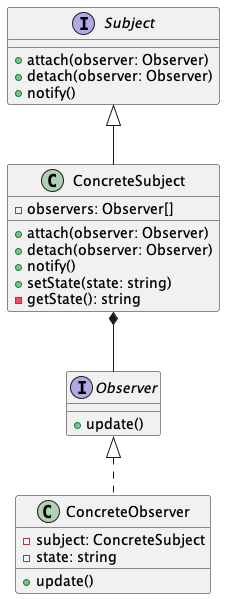
\includegraphics[width=0.18\textwidth]{fig/uml/default-observer.png}
    \caption{Einfaches Observer Pattern}
    \label{fig:default-observer}
  \end{figure}
\end{frame}

\begin{frame}
  %\frametitle{Observer}
  \framesubtitle{Pattern Beispiel Lampe - Architektur}
  \begin{figure}[ht]
    \centering
    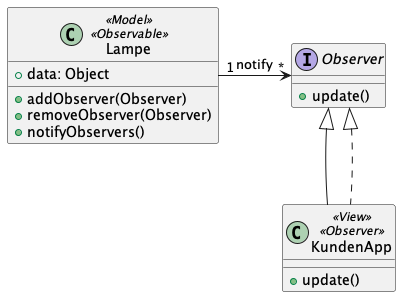
\includegraphics[width=0.65\textwidth]{fig/uml/mvc-observer.png}
    \caption{Observer Pattern als Verbindung zwischen Model und View}
    \label{fig:mvc-observer}
  \end{figure}
\end{frame}

\begin{frame}
  \frametitle{Observer}
  \framesubtitle{Pattern Beispiel Lampe - Verhalten}
  \begin{figure}[ht]
    \centering
    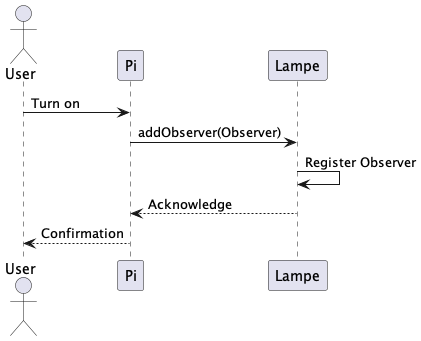
\includegraphics[width=0.55\textwidth]{fig/uml/seq-mvc-observer.png}
    \caption{Observer Pattern als Verbindung zwischen Model und View}
    \label{fig:seq-mvc-observer}
  \end{figure}
\end{frame}

\begin{frame}
  \frametitle{Observer}
  \framesubtitle{Im Kontext von MVC und VS}
  \begin{itemize}
    \item Nicht nur eine Design-Frage
    \item Technologie-abhängig
    \item Uni-direktionalen Kommunikation zwischen dem Subjekt und den Beobachtern
    \item Request-Response-Cycle unterstützt Observer nicht direkt
    \item WebSockets, Long Polling, HTTP2 oder HTTP3 können Optionen anbieten
  \end{itemize}
\end{frame}